\documentclass[conference]{IEEEtran}

\ifCLASSOPTIONcompsoc
  \usepackage[nocompress]{cite}
\else
  \usepackage{cite}
\fi

\usepackage[pdftex]{graphicx}
\graphicspath{{../img/}}

\begin{document}

\title{Parceive\\The Paper}

\author{A. Wilhelm,
		V. Savu
        and~E. Amadasun}% <-this % stops a space

\IEEEtitleabstractindextext{%
\begin{abstract}
Since the advent of multicore processors developers struggle with the parallelization
of legacy software. Automatic methods are appropriate to identify parallelism on
instruction level or simple loops. However, a scalable refactoring additionally requires
profound comprehension of the given software architecture and its dynamic aspects. This
leads to a rising demand for interactive tools to foster parallelization at various
granularity levels. To alleviate this problem, we propose a visualization framework, and
two tailored views for parallelism detection. This framework builds upon Parceive, our
tool that utilizes dynamic binary instrumentation to trace C/C++/C\# programs. The
cooperative views allow the identification and analysis of potential parallelism
scenarios. Seamless navigation, abstraction, and filtering ensure an effective aid in
comprehending legacy software. In this paper, we motivate our approach, illustrate the
architecture of our visualization framework, and highlight the key features of our
views. A case study shows the usefulness of Parceive.
\end{abstract}

\begin{IEEEkeywords}
Computer Society, IEEE, IEEEtran, journal, \LaTeX, paper, template.
\end{IEEEkeywords}}

\maketitle

\IEEEdisplaynontitleabstractindextext
\IEEEpeerreviewmaketitle

\section{Introduction}
\label{sec:introduction}
The advent of multicore processors still poses a big challenge to the industry and
the research community. To exploit the increasing processing power of such systems
software parallelism is indispensable. As a result, software vendors are forced to
parallelize their legacy software to make them scalable. Such a parallelization
relies on two essential steps. The first step is to sufficiently comprehend the
given software structure and its dynamic behaviour. The second step is a potential
redesign of the software architecture that enables parallelism. Unfortunately, both
steps are tedious and error-prone so that most of the legacy software still operates
sequentially. Besides the additional complexity of parallel programming, we believe
the problem largely arises due to a lack of appropriate tool support.

\todo{[Paragraph about dynamic analysis vs. static approaches]}

\todo{[Paragraph about contributions]}

\todo{[Paragraph about outline]}

\section{Parceive}
\label{sec:parceive}
We implemented Parceive, a tracing-based tool for interactive software
analysis. Its vision is to aid developers with identifying parallelism opportunities
on various granularity levels. Parceive utilizes static binary analysis and dynamic
instrumentation to collect trace data. Being less conservative than pure static
approaches let us focus on concurrency-related events, e.g., memory accesses, routine
invocations, and object instantiations. A-posteriori abstraction of such fine-grained
information enables to infer architectural aspects of user applications. Here is the
difference to most existing tools, the results may be used as a starting point for an
extensive architecture refactoring. However, the user is responsible for a correct
parallelization due to the inherent incompleteness of dynamic analysis.

\begin{figure}
\begin{center}
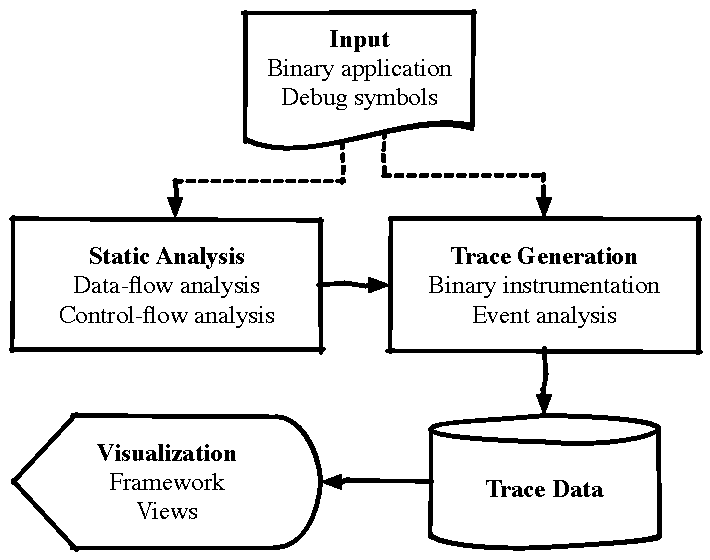
\includegraphics[width=0.45\textwidth]{img/parceive}
\caption{Overview of Parceive}
\end{center}
\end{figure}

The visualization component of Parceive is the user's key to comprehend and parallelize
their applications. The component allows to grasp complex system behaviour by providing
selective views for different viewpoints. Each view tries to simplify and
highlight specific aspects of the traced software. Examples are a performance view to
detect hotspots, or a function view that depicts memory dependencies between functions.
The biggest challenge when dealing with runtime traces is the potentially overwhelming
amount of data. Often such traces lead to unmanageable visualizations with unpractical
delays. We address this problem by providing three key services to each view. The first
service allows on-demand loading of arbitrary trace data and its caching for reuse
across views. Most importantly, this service enables users to navigate and explore
their software. The second service is the abstraction of fine-grained trace information
to high-level entities, e.g., from single function invocations to call-groups, or from
objects to classes. Such abstractions allow to comprehend software by using scalable
top-down approaches. The third service comprises a communication infrastructure for
sharing arbitrary state across multiple views. This service can be used to spot and
restrict the current range of view to crucial points in the trace.  Equipped with all
these services (and additional, highly optimized queries) the visualization component
allows scalable views for software analysis.

\subsection{System Architecture}
\label{sec:system_architecture}

\subsection{Data Model}
\label{sec:data_model}

\subsection{Data Extraction}
\label{sec:data_extraction}

\section{Views}
\label{sec:views}

\subsection{Profiling View}
\label{sec:profiling_view}

\subsection{CCT View}
\label{cct_view}

\section{Case Studies}
\label{sec:case_studies}

\subsection{CppCheck}
\label{sec:cppcheck}

\subsection{TensorFlow}
\label{sec:tensorflow}

\section{Discussion}
\label{sec:discussion}

\section{Related Work}
\label{sec:related_work}

\subsection{Software Comprehension}
\label{sec:software_comprehension}

\subsection{Parallelization}
\label{sec:related_work_parallelization}

\section{Conclusion}
\label{sec:conclusion}

\section{Framework}

\subsection{Database processing}
\label{dataprocessing}

The database layout and settings used by Parceive are highly optimized for fast writing. All the information required by the visualization can be obtained by using queries, but most of the operations will take a disproportionate amount of time to complete.

The first problem with the database is that Parceive avoids the creation of indexes to improve write performance. Thus, the most important step of the database processing is the creation of multiple indexes to improve record lookup. All primary and foreign keys are indexed and some composite indexes are created to speed up specific queries.

Since no additional data will be added to the database, creating redundancy generates no overhead and does not increase the complexity. By adding additional fields and creating intermediary tables, it is possible to avoid joins for most queries executed by the visualizations. 

Executing \texttt{VACUUM} after all processing is done also improves performance by reducing the fragmentation of data stored inside tables. The increased locality of data reduces the execution time of most queries and has a considerable effect on ones that require a full table scan. \texttt{VACUUM} is also able to reduce the size of the processed database.

\subsubsection*{Performance}

Figure \ref{parceive:procperformance} shows the time and size overhead of processing databases generated by Parceive. The time required by this operation is negligible because loading most visualizations without the optimizations would waste more than the processing itself. The executed queries are also heavily optimized making \texttt{VACUUM} and the creation of indexes the most time consuming operations. The size increase is unfortunately unavoidable.

\begin{figure}
	\centering
	\begin{tabular}{l l l l}
		Database & Size & Processed Size & Time taken \\
		emsim\_par & 3905536 & 14560256 & 8.77 s
	\end{tabular}
	\caption{Database processing performance}
	\label{parceive:procperformance}
\end{figure}

\subsection{NodeJS Server}

Loading the entire database into the browser is not possible when the trace is too large. To solve this problem a simple NodeJS Server was developed to read data from a processed database on demand.

The server exposes a very simple REST \cite{rest} API that only allows the retrieval of data. For security reasons all SQL queries are contained in this server and  arbitrary queries are not supported. The implementation makes use of multiple parallel reads to the same database to reduce the latency and throughput when large amounts of data is requested by the visualizations.

\subsection{ORM}

Visualizations developed within the Parceive architecture can employ a Object Relational Mapper to simplify development and improve performance. The ORM makes it possible to access entities and to easily navigate the relationships between them. The API is implemented using promises \cite{promises} simplifying the asynchronous and parallel behavior.

The greatest benefit to using this ORM in visualizations is the possibility of applying optimizations to the data loading. The most important ones are caching and pipelining.

Caching allows the ORM to avoid loading data that has been accessed before. Each time an entity is retrieved from the server it is saved and reused for subsequent requests. This optimization allows visualizations to focus more on data presentation instead of efficient data retrieval.

Pipelining combines multiple queries to the same endpoint into a single one. When requesting a large number of entities it can improve performance despite the limit on the number of parallel requests in browsers. This optimization is designed to greatly increase throughput at the cost of a response time increased by 10 milliseconds.

\subsection{Visualization Framework}

As part of the Parceive UI a visualization framework has been developed to handle the layout and communication of multiple visualizations. The implementation is based on AngularJS and it completely separates visualizations into separate applications.

\subsubsection{State management}

The visualization framework implements a centralized and persistent state storage for visualizations. With the use of this feature it is possible to retain the state of views across page loads.

Currently the view layout and the marked nodes are stored as part of the state automatically. In addition to this each visualization can save tailored information at any time and retrieve it when rendering. Local storage is used to house all the state information making it persistent.

\subsubsection{Communication}

Visualizations perform different tasks and allow the user to navigate the callgraph in different ways. Communication makes it possible to follow a chain of investigation along multiple visualizations. Currently there are three ways to communicate intent:

\begin{itemize}
	\item[Focus] brings entities to the attention of the user
	\item[Mark] allows the creation of selections that are visible between visualizations
	\item[Spot] replaces all the entities in a visualization with a new set
	\item[Hover] brings entities to the attention of the user using opacity
\end{itemize}


\section{Visualizations}

\subsection{Source View}

The source view is the simplest visualization developed for Parceive. It shows the highlighted source code in a file that was used to build the instrumented application.

The usefulness of this view only becomes apparent when it is communicating with the others presented in this paper. The simplest interaction is focusing and it allows the source view to pinpoint the definition of functions an loops making it easy to follow the execution of a program trough the source code.

Hovering is able to provide additional information about entities. For calls it can indicate where the call originated and for memory references where they were allocated and referenced.

\subsection{Calling context tree View}

The CCT View is a visualization that allows an user to easily comprehend the dynamic behavior of an application. It can display and easily navigate Calls, Loops and References.

The first node present when the view is created is the call to \texttt{main}. The user can then expand it like any other call by clicking or using the context menu. When a function is called multiple times the calls are grouped into a CallGroup to reduce the number of nodes displayed. CallGroups can be easily decomposed into their Calls by using the context menu.

Loops can be visually identified by icons on nodes. When a loop icon is present on the right side of a node then that node contains one or more loops. These loops can be added to the visualization by using the context menu. A icon on the left side indicates that the call has been made from inside a loop. Navigating loop executions and loop iterations is similar to calls and allows the user to see information at any granularity he desires.

CallGroups, Calls, LoopExecutions and LoopIterations are positioned using the D3 tree layout. Children of a node are always sorted by their start time. This positioning of nodes creates a clear indicator of the relationship between them.

References accessed by parts of the application can be displayed by using the context menu. These nodes are difficult to integrate as part of a graph layout and are positioned using a force simulation around the rest of the tree.

This view has some additional features that aim to help a developer parallelize code:

\begin{itemize}
	\item Profiling information is present as the node color
	\item References shared between nodes can be easily identified
	\item It is easy to expand the references accessed during the inclusive execution of a call or callgroup
	\item A specialized query that only display the shared references between nodes
\end{itemize}

\appendices
\section{Proof of the First Zonklar Equation}
Appendix one text goes here.

% you can choose not to have a title for an appendix
% if you want by leaving the argument blank
\section{}
Appendix two text goes here.

% Can use something like this to put references on a page
% by themselves when using endfloat and the captionsoff option.
\ifCLASSOPTIONcaptionsoff
  \newpage
\fi

\end{document}


